% =================================================================================
\section{Approximation par la méthode de Galerkin-Discontinu}
% =================================================================================
La méthode de Galerkin-Discontinu fait un lien entre les méthodes de volumes finis et d'éléments finis. En effet, on commence par écrire la formulation variationnelle et ensuite comme en élément fini on approche la solution théorique par une solution discrète à l'aide d'une combinaison linéaire de fonctions de base. \\
Même si les fonctions tests et les fonctions de base sont dans le même espace aucune continuité n'est imposé aux interfaces entre les éléments du maillage.
Nous prendrons une base polynomiale obtenu par un développement de Taylor. Il existe différent choix possible mais celui-ci permet une approche plus simple en ignorant la géométrie des mailles comme nous le verrons plus tard. \\
Nous allons commencer par étudier le cas $P_0$ où notre base est uniquement composée de la fonction constante égale à $1$, on retrouvera alors le schéma d'Euler implicite étudié précédemment. Puis, on pourra passer agrandir notre base en passant en $P_1$. Toute cette section s'inspire fortement des sources \cite{DiPietro2012}, \cite{FrancoisVilar2010} et \cite{Gerald2014}.
\\
On commence par partir du problème de Rayleigh-Stokes $1$D homogène
\begin{equation}
    \begin{cases}
        \partial_tu(t,x) - \nu\partial_{xx} u(t,x) - \alpha\partial_{txx} u(t,x) = 0 & (t,x) \in \mathbb R_+ \times \bbR  \\
        u(0,x) = u_0(x) & x \in \bbR
    \end{cases}
\end{equation}
On cherche alors a effectuer une formulation faible du problème en multipliant par une fonction test $v$ suffisamment régulière. En se plaçant sur une maille $K_i$ on peut alors écrire
\begin{equation*}
   \int_{K_i} \partial_t uv - \nu \int_{K_i}\partial_{xx}uv \ - \alpha \int_{K_i} \partial_{txx}uv = 0
\end{equation*}
En utilisant une formule de Green on obtient le résultat suivant
\begin{equation*}
    \int_{K_i} \partial_t uv + \nu \int_{K_i}\partial_{x}u\partial_{x}v \ + \alpha \int_{K_i} \partial_{tx}u\partial_{x}v
    =  \nu \int_{\partial K_i}(\partial_{x}u \cdot n)v \ + \alpha \int_{\partial K_i} (\partial_{tx}u \cdot n)v
\end{equation*}
Ce qui donne dans le cas $1$D
\begin{equation}\label{EDP_RS_Formulation_Faible}
    \int_{K_i} \partial_t uv + \nu \int_{K_i}\partial_{x}u\partial_{x}v \ + \alpha \int_{K_i} \partial_{tx}u\partial_{x}v
    =  \nu \Big[\partial_{x}u v \Big]^{x_i +h/2}_{x_i - h/2} \ + \alpha \Big[\partial_{tx}u v \Big]^{x_i +h/2}_{x_i - h/2} 
\end{equation}
Cette équation change grandement selon le choix de la base, par exemple pour une méthode Galerkin discontinu d'ordre 2, on obtient en faisait un développement de Taylor 
\begin{equation*}
    u(X) = u(X_i) + (X - X_i)\partial_X u(X_i) + \mathcal{O}\!\left((X - X_i)^2\right)
\end{equation*}
avec $X_i$ désignant le centroïde d'une cellule de longueur $h$.

Calculons la valeur moyenne $\bar{u}_i$ de notre inconnue sur une maille $K_i$
\begin{equation*}
\bar{u}_i = \frac{1}{h} \int_{K_i} u(X)\,dX = u(X_i) + \mathcal{O}\!\left(h^2\right)
\end{equation*}
Par conséquent
\begin{equation*}
u(X) = \bar{u}_i + h\,\partial_X u(X_i)\,\frac{X - X_i}{h} + \mathcal{O}\!\left(h^2\right)
\end{equation*}
On choisit alors la base $\{e_0, e_1\} = \left\{1, \dfrac{X - X_i}{h}\right\}$.
Le problème consiste donc à trouver $u_{h_{|K_i}} := u_h^i$, l'approximation de $u$ sur $K_i$, comme fonction de $\mathcal{P}^1(K_i)$ dans la base $\{e_j^i\}_{j=0,1}$ sous la forme 
\begin{equation}\label{base_formulation_varia_GD}
    u_h^i = \sum_{j=0}^{K} u_j^i(t)\, e_j^i(X) = u_0^i(t) + u_1^i(t)\,\frac{X - X_i}{h}
\end{equation}
Toute cette partie est bien écrite dans \cite[p.~29]{FrancoisVilar2010}.

\subsection{Etudes selon la taille de la base}
\subsubsection{Le cas \texorpdfstring{$P_0$}{P0}}
Dans le cas où l'on se contente de considérer la base  $\{e_0\} = \{ 1 \}$, on peut simplifier \eqref{EDP_RS_Formulation_Faible} qui prend en compte des $\partial v$ qui vaut $0$.
L'équation devient:
\begin{equation*}
    \int_{K_i} \partial_t u =  \nu \Big[\partial_{x}u \Big]^{x_i +h/2}_{x_i - h/2} \ + \alpha \Big[\partial_{tx}u \Big]^{x_i +h/2}_{x_i - h/2} 
\end{equation*}
En reprenant la formulation \eqref{base_formulation_varia_GD} cela se réécrit plus simplement:
\begin{equation}\label{EDP_RS_Formulation_Faible_P0}
    h\ \partial_t u_0^i = \nu \Big(\partial_{x}u_h^i\big|_{x_i + h/2} - \partial_{x}u_h^i\big|_{x_i - h/2} \Big) \ + \alpha \Big(\partial_{tx}u_h^i\big|_{x_i + h/2}- \partial_{tx}u_h^i\big|_{x_i - h/2}\Big) 
\end{equation}
\\
En reprenant la formulation \eqref{EDP_RS_Formulation_Faible_P0} il nous faut alors correctement définir le flux numérique. La trace $\partial_{x}u_h^i\big|_{x_i + h/2}$ n'est pas unique et est défini de chaque côté de l'interface. En $P0$ elle est même nulle puisque $u_h^i = u_0^i$ qui est constant sur les mailles. Donc on va ajouter un terme de pénalisation et utiliser le saut au niveau de chaque maille (voir \cite{DiPietro2012} page 125). Soit $\eta = 1$, on obtient alors:
\begin{equation*}
    \partial_x u_h\big|_{x_i + h/2} = \eta \frac{u_0^{i+1} - u_0^i}{h}, \qquad
    \partial_x u_h\big|_{x_i - h/2} = \eta \frac{u_0^i - u_0^{i-1}}{h}
\end{equation*}
En injectant dans l'équation on alors:
\begin{equation*}
    h\,\partial_t u_0^i = \nu\left(\frac{u_0^{i+1} - u_0^i}{h} - \frac{u_0^i - u_0^{i-1}}{h}\right)
    + \alpha\left(\frac{\partial_t u_0^{i+1} - \partial_t u_0^i}{h} - \frac{\partial_t u_0^i - \partial_t u_0^{i-1}}{h}\right)
\end{equation*}
ce qui se simplifie en :
\begin{equation*}
    h\,\partial_t u_0^i = \frac{\nu}{h}\left(u_0^{i+1} - 2u_0^i + u_0^{i-1}\right)
    + \frac{\alpha}{h}\left(\partial_t u_0^{i+1} - 2\partial_t u_0^i + \partial_t u_0^{i-1}\right)
\end{equation*}

En divisant par h on reconnaît exactement le schéma en différences finies :
\begin{equation*}
    \partial_t u_i - \nu\Delta_h u_i - \alpha\Delta_h\!\left(\partial_t u_i\right) = 0
\end{equation*}
où $\Delta_h u_i = \dfrac{u_{i+1} - 2u_i + u_{i-1}}{h^2}$. \\
On résout alors le problème de façon similaire au chapitre \ref{Chapitre_3}. Numériquement, les résultats sont similaires :
\begin{figure}[H]
    \centering
    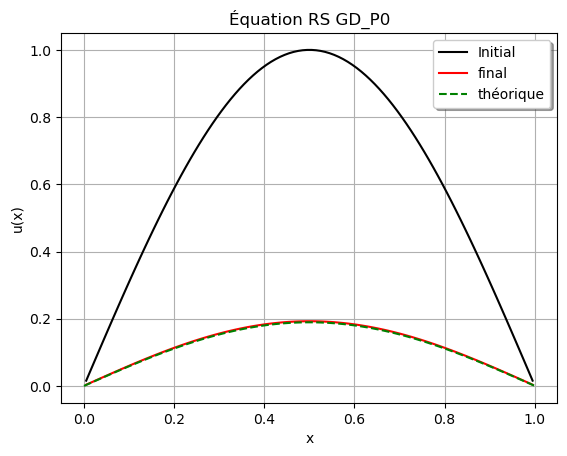
\includegraphics[width=0.5\linewidth]{images/DG/P0.png}
    \caption{Résolution par GDP0}
    \label{GDP0}
\end{figure}

\subsubsection{Le cas \texorpdfstring{$P_1$}{P1}}
On prend désormais la base $\{\phi_0, \phi_1\} = \left\{1,\  \dfrac{X - X_i}{h}\right\}$. La solution approché $u_h$ s'écrit (dans cette base et sur la i-ème maille): $ u_h = u^0_i \phi_0 + u^1_i \phi_1$. \\
En remplaçant cette nouvelle expression dans \ref{EDP_RS_Formulation_Faible} on obtient (Pour $j = 0 , 1$):
\begin{eqnarray*}\label{EDP_RS_Formulation_Faible_P1}
  &\partial_t u_i^0 \int_{K_i}  \phi_0 \phi_j + \partial_t u_i^1 \int_{K_i}  \phi_1 \phi_j& \\
   &+\nu \ u_i^0  \int_{K_i}\partial_{x}\phi_0 \partial_{x}\phi_j  + \nu \ u_i^1 \int_{K_i}\partial_{x}\phi_1 \partial_{x}\phi_j& \\
   &+ \alpha \partial_{t}u_i^0 \int_{K_i} \partial_{x}\phi_0\partial_{x}\phi_j + \alpha \partial_{t}u_i^1 \int_{K_i} \partial_{x}\phi_1\partial_{x}\phi_j &\\
    &=& \\ 
    &\nu \Big[\partial_{x}\big(u_i^0\phi_0 +u_i^1\phi_1 \big) \phi_j  \Big]^{x_i +h/2}_{x_i - h/2} \ + \alpha \Big[\partial_{tx}\big(u_i^0\phi_0 +u_i^1\phi_1 \big) \phi_j \Big]^{x_i +h/2}_{x_i - h/2} 
\end{eqnarray*}
On calcule les matrices de l'expression précédente.
\begin{eqnarray*}
    &&\int_{K_i}  \phi_0 \phi_0 = \int_{K_i}  1 = h \\
    &&\int_{K_i}  \phi_0 \phi_1 = \int_{K_i} \frac{x -x_i}{h} = 0 \\
    &&\int_{K_i}  \phi_1 \phi_1 = \int_{K_i} \bigg(\frac{x -x_i}{h}\bigg)^2 = \frac{h}{12} \\
    &&\int_{K_i}  \partial\phi_0 \partial\phi_0 = \int_{K_i}  \partial\phi_0 \partial\phi_1= 0 \\
    &&\int_{K_i}  \partial\phi_1 \partial\phi_1 = \frac{1}{h^2} 
\end{eqnarray*}

Il nous faut alors encore traiter les valeurs aux interfaces correctement. Cette fois la trace du gradient de $u_h$ ne s'annule pas et vaut $\frac{u_i^1}{h}$ sur la maille $K_i$ et  $\frac{u_{i+1}^1}{h}$ sur la maille $K_{i+1}$
On définit alors le flux moyen à chaque interface (qui va remplacer la trace du gradient) comme: $\{\!\!\{ u_i^1 \}\!\!\}_{F_i} = \frac{u_{i}^{1} + u_{i+1}^{1}}{2h}$ où $F = K_i \cap K_{i+1}$ \\
Maintenant que tout est bien défini on peut écrire le système suivant:

\begin{eqnarray*}
    &&\begin{bmatrix}
        h & 0 \\
        0 & \frac{h}{12} 
    \end{bmatrix}
    \begin{bmatrix}
    \partial_t u_i^0 \\
    \partial_t u_i^1    
    \end{bmatrix}
    +
        \begin{bmatrix}
        0 & 0 \\
        0 & \frac{\nu + \alpha \partial_t}{h} 
    \end{bmatrix}
    \begin{bmatrix}
    u_i^0 \\
    u_i^1    
    \end{bmatrix}
    = (\nu + \alpha\partial_t)
    \begin{bmatrix}
    \{\!\!\{ u_i^1 \}\!\!\}_{F_i} - \{\!\!\{ u_i^1 \}\!\!\}_{F_{i-1}}\\
    \{\!\!\{ u_i^1 \}\!\!\}_{F_i} \times\frac{1}{2} - \{\!\!\{ u_i^1 \}\!\!\}_{F_{i-1}} \times (- \frac{1}{2})
    \end{bmatrix} \\
    \\
    &&\begin{bmatrix}
        h & 0 \\
        0 & \frac{h}{12} 
    \end{bmatrix}
    \begin{bmatrix}
    \partial_t u_i^0 \\
    \partial_t u_i^1    
    \end{bmatrix}
    +
        \begin{bmatrix}
        0 & 0 \\
        0 & \frac{\nu + \alpha \partial_t}{h} 
    \end{bmatrix}
    \begin{bmatrix}
    u_i^0 \\
    u_i^1    
    \end{bmatrix}
    = (\nu + \alpha\partial_t)
    \begin{bmatrix}
    \frac{u_{i+1}^1 - u_{i-1}^1 }{2h}\\
    \frac{u_{i+1}^1 - u_{i-1}^1 }{4h}
    \end{bmatrix}
\end{eqnarray*}
Qui se réécrit plus simplement :
\begin{eqnarray*}
    M \partial_t U + C U = B
\end{eqnarray*}

Pour approcher la dérivée en temps on utilise Euler Explicite. On pourra alors calculer la solution $U$ au temps $n+1$ en fonction de $U$ au temps $n$ sur une maille $K_i$.\\
Cette approche est certainement trop brutale car elle ne permet pas d'adapter facilement la montée en ordre de la méthode ce qui est sensé être un des avantages de Galerkin Discontinu. Il faut certainement repartir de la formulation variationnelle et réussir à exprimer ça de façon plus générale...

On trouve un exemple qui correspond à une version simplifié de notre équation dans "\cite{Gerald2014}" (page 193 à 196)
"Un premier choix dit « naïf », pour le flux numérique de la dérivée spatiale est un flux numérique centré". Notre façon de faire et donc simpliste et peut présenter des problèmes plus tard mais reste une première approche acceptable.
% Je trouve ça un peu partout:Le terme de bord issu de l'IPP sur $K_i$ s'écrit, en utilisant le flux numérique centré
%$\widehat{\sigma}_{i\pm 1/2} := \{\{ \partial_x u_h \}\}_{ i \pm 1/2}$:

















